\documentclass[10pt,a4paper]{article}
\pdfsuppressptexinfo=-1
\usepackage[T1]{fontenc}
\usepackage{lmodern}
\usepackage[margin=0.66in]{geometry}
\usepackage[compact]{titlesec}
\titlespacing*{\section}{0pt}{8pt}{3pt}
\titleformat*{\section}{\large\bfseries}
\setlength{\textfloatsep}{8pt}
\setlength{\floatsep}{6pt}
\setlength{\intextsep}{6pt}
\usepackage{amsmath,amssymb,bm}
\usepackage{booktabs,array}
\usepackage{graphicx}
\usepackage{tikz}
\usetikzlibrary{arrows.meta,positioning}
\usepackage[font=small,labelfont=bf]{caption}
\usepackage[hidelinks,pdfcreator={},pdfproducer={}]{hyperref}
\usepackage{enumitem}
\usepackage{multicol}
\setlist{nosep,leftmargin=1.2em}
\setlength{\parskip}{3pt}

\title{\vspace{-2.4em}\large\textbf{Learning for the Decision: Replicating and Extending End-to-End\\Markowitz Learning in China's A-Share Market}}
\author{\normalsize Kumar Utkarsh, Indian Institute of Technology Guwahati}
\date{\small Working draft, October 2026\vspace{-1.2em}}

\newcommand{\rhat}{\hat{\bm r}}
\newcommand{\w}{\bm w}

\begin{document}
\maketitle
\vspace{-1.2em}

\begin{abstract}
\noindent Portfolio construction usually separates return prediction from optimization: a model is fit to
minimize mean squared error and its forecasts are then passed to an optimizer. Wang, Gao, Harvey, Liu and Tao
(2026) argue that this separation is costly and propose end-to-end (E2E) training, in which the optimizer is a
differentiable layer and the network is trained on the realized portfolio objective. We replicate their design on
the same market (daily China A-shares, 2010 to 2023) using only free data, audit the paper's internal
consistency, and extend it. We derive exact differentiable layers for the paper's portfolio problems, fit
closed-form linear and dimension-reduction models (ridge, PCR, PLS, LDA), and propose decision-aware dimension
reduction. We also show that, without tradability rules the paper does not state, much of the long-only
return comes from newly listed stocks locked at their upper price limit, which cannot be bought. Out of sample
over 2014 to 2023, end-to-end training lowers statistical accuracy but raises long-only returns, most for models
that are weak under MSE; decision-aware PCA lifts a 20-component linear model from a Sharpe ratio of 1.00 to 1.36
($t=5.0$). With 20 bps costs, end-to-end training cuts daily turnover from 28\% to 7\%, but its edge over a
validation-tuned cost-aware benchmark is not significant.
\end{abstract}

\section{Introduction}
The standard ``predict, then optimize'' approach treats forecast errors as equally important for every stock. A
long-only investor holding the top decile, however, cares about accuracy only near the top of the ranking, and
an investor facing trading costs cares about signals that do not force turnover. Wang et al.\ (2026) embed the
portfolio problem in training so that the prediction model learns what the decision needs, and report that this
raises long-only returns, survives transaction costs and traces a better efficient frontier. Our contributions are:
\begin{enumerate}
\item A reproducible replication on free data that covers the paper's market, frequency, universe filters,
  VWAP execution and industry classification (Section~\ref{sec:data}).
\item An audit of the paper: conventions it does not state but its tables imply, numbers that contradict each
  other, and claims the tables do not support, each with a resolution (Section~\ref{sec:audit}).
\item An exact differentiable portfolio layer with an $O(N)$ closed-form Jacobian (Section~\ref{sec:layer}).
\item Extensions in the prediction layer: closed-form linear and dimension-reduction models, decision-aware
  PCA, and mixture-of-experts models (Section~\ref{sec:ext}).
\item Full out-of-sample results for E2E training, decision-aware PCA, transaction costs and mean--SD utility,
  each tested against its own two-stage starting point (Section~\ref{sec:results}).
\end{enumerate}

\section{Data and replication design}\label{sec:data}
We combine two free Qlib-format dumps of Tushare data. The first provides raw daily prices, VWAP, adjustment
factors, market capitalization, price limits, ST intervals, Shenwan level-1 industries and 163 point-in-time
financial indicators with announcement dates, for 5,490 stocks including delisted ones. The second supplies
2007 to 2009 price history and the CSI 500 index. An independent JoinQuant copy confirms the daily VWAP returns
(correlation 0.9995 over 479,000 stock-days). Table~\ref{tab:setup} compares the design with the paper's.

\begin{table}[h]
\centering\small
\caption{Replication design.}\label{tab:setup}
\begin{tabular}{p{2.6cm}p{6.2cm}p{6.6cm}}
\toprule
& Wang et al.\ (2026) & This study \\
\midrule
Sample & A-shares 2010--2023, 5.96M stock-days & A-shares 2010--2023, 10.04M stock-days, 2,953 stocks/day \\
Target & VWAP$(t{+}1)\to$VWAP$(t{+}2)$ minus CSI 500 & Same (index leg close-to-close over day $t{+}2$) \\
Universe & excludes ST and suspended stocks & Same, on decision day $t$ \\
Tradability & not discussed & drop a stock's first 60 trading days and days locked at the upper limit on $t{+}1$ \\
Characteristics & 415 daily, 31 Shenwan industries & 47 price/volume, 163 fundamental, 10 valuation, 31 Shenwan \\
Windows & 39m train, 9m validation, 3m test, quarterly roll & Same, 40 windows (2014Q1--2023Q4), 2-day embargo \\
\bottomrule
\end{tabular}
\end{table}

\section{Methodology}
\paragraph{Two-stage benchmark.} Stock $i$'s market-adjusted return is modeled as $r_{i,t+1}=g(\bm x_{i,t};\bm\theta)
+\epsilon_{i,t+1}$, with $g$ linear or a feed-forward network (NN1 to NN5, layers 32-16-8-4-2), fit by
$\min_{\bm\theta}\frac{1}{NT}\sum_{i,t}(r_{i,t+1}-g(\bm x_{i,t};\bm\theta))^2$ with Adam and early stopping. Each
day the forecasts are sorted into deciles; the long-only portfolio holds the top decile.

\paragraph{End-to-end learning.} E2E solves the bilevel problem
\begin{equation}
\min_{\bm\theta}\;\frac1T\sum_{t}\Big[-\w_t^{\star\top}\bm r_{t+1}+\tfrac{\gamma}{2}\lVert\w_t^\star-\w_{t-1}^\star\rVert_1\Big],
\quad
\w_t^\star=\arg\min_{\w\in\mathcal W_t}\;-\w^\top\rhat_{t+1}+\zeta\lVert\w\rVert_2^2+\tfrac{\gamma}{2}\lVert\w-\w^\star_{t-1}\rVert_1,
\label{eq:bilevel}
\end{equation}
with $\rhat_{t+1}=g(\bm x_t;\bm\theta)$ and $\mathcal W_t=\{\w:\bm 0\le\w\le u_t\bm 1,\ \bm 1^\top\w=1\}$, where
$u_t=1/(0.1N_t)$ so that the unregularized solution is the equal-weighted top decile. The term $\zeta\lVert\w\rVert^2$
smooths the otherwise piecewise-constant solution of the linear program, and $\gamma$ is the transaction cost
rate. The gradient follows the chain rule $\nabla_{\bm\theta}=\sum_t(\partial\rhat/\partial\bm\theta)^\top
(\partial\w^\star/\partial\rhat)^\top\partial f_u/\partial\w^\star$.

\paragraph{An exact differentiable portfolio layer.}\label{sec:layer} The paper differentiates the lower level
through its KKT conditions with a generic solver. For problem~\eqref{eq:bilevel} this is unnecessary. The
objective is separable apart from the budget constraint, so with multiplier $\tau$ each weight solves a
one-dimensional problem:
\begin{equation}
w_i^\star=\Pi_{[0,u]}\!\big(S_{p_i}(\hat r_i-\tau)\big),\qquad
S_p(a)=\begin{cases}(a-c)/2\zeta & a>2\zeta p+c\\ (a+c)/2\zeta & a<2\zeta p-c\\ p & \text{otherwise}\end{cases},\quad c=\gamma/2,
\label{eq:layer}
\end{equation}
where $p_i$ is yesterday's weight and $\tau$ is the unique root of $\sum_i w_i^\star(\tau)=1$, found by bisection.
With $\gamma=0$ this is the Euclidean projection of $\rhat/2\zeta$ onto the capped simplex. Let $F$ be the set of
stocks strictly inside their bounds and off the plateau at $p_i$. Differentiating the budget identity gives
\begin{equation}
\frac{\partial\w^\star}{\partial\rhat}=\frac{1}{2\zeta}\Big(\bm D_F-\frac{\bm 1_F\bm 1_F^\top}{|F|}\Big),
\label{eq:jac}
\end{equation}
with $\bm D_F$ the diagonal indicator of $F$. The backward pass is therefore $O(N)$: subtract the mean upstream
gradient over $F$ and scale. We verified~\eqref{eq:layer} against a general solver (60 random problems, gap below
$10^{-17}$) and~\eqref{eq:jac} against finite differences (relative error $10^{-11}$).

\paragraph{Evaluation.} We follow conventions recovered from the paper's tables (Section~\ref{sec:audit}): H--L is
$(H-L)/2$; turnover is $\tfrac12\lVert\w_t-\w_{t-1}\rVert_1$ and costs are $\gamma$ times turnover; returns are
annualized with 243 trading days; tests use Newey--West errors with $\lfloor T^{1/4}\rfloor$ lags.

\section{Extensions in the prediction layer}\label{sec:ext}
\paragraph{Closed-form linear family.} Every linear model predicts with one vector $\bm\beta$, so it can be fit
from a window's sufficient statistics $\{n,\sum\bm x,\bm X^\top\bm X,\bm X^\top\bm y,\text{class sums}\}$,
accumulated on the GPU in one pass. With $\bm C$ and $\bm c$ the centered covariances:
ridge $\bm\beta=(\bm C+\lambda\bar\sigma^2\bm I)^{-1}\bm c$; principal components regression
$\bm\beta=\bm V_K(\bm V_K^\top\bm C\bm V_K)^{-1}\bm V_K^\top\bm c$; PLS via SIMPLS on $(\bm C,\bm c)$; and Linear
Discriminant Analysis with classes given by each day's return deciles, solving $\bm S_b\bm v=\lambda\bm S_w(\alpha)\bm v$
with $\bm S_w(\alpha)=(1-\alpha)\bm S_w+\alpha\,\mathrm{tr}(\bm S_w)/p\,\bm I$, then regressing on the top $m$
directions. A ``top decile versus rest'' Fisher discriminant targets the long-only decision directly.
Hyperparameters are chosen per window on validation rank IC, and every setting tried is reported.

\paragraph{Decision-aware dimension reduction.} For a linear model a learned linear bottleneck adds nothing,
since $(\bm W\bm\gamma)^\top\bm x$ is still one linear score. Reduction matters only as a constraint, so we
propose
$\min_{\bm\theta,\bm W}\ \mathcal L_{\mathrm{dec}}(\bm\theta,\bm W)+\mu\lVert\bm W-\bm V_K\rVert_F^2$, which
starts from the PCA loadings and lets the portfolio objective move them; $\mu\to\infty$ gives PCA followed by E2E.
For the networks the bottleneck feeds nonlinear layers and changes the function class. A persistence-aware
variant chooses directions that minimize $\bm v^\top\bm C_\Delta\bm v/\bm v^\top\bm C\bm v$, with $\bm C_\Delta$ the
covariance of daily changes, favouring slow, low-turnover signals for the cost experiment.

\paragraph{Mixtures and robust losses.} A Gaussian mixture on PCA scores gives memberships $\pi_k(\bm x)$ and linear
experts $g(\bm x)=\sum_k\pi_k(\bm x)\bm x^\top\bm\beta_k$, as in the paper's example where large and small firms
price differently. Linear and random-Fourier-feature SVR give robust and nonlinear baselines.

\section{Auditing the original paper}\label{sec:audit}
Table~\ref{tab:audit} lists the most consequential findings; each numeric item was recomputed from the paper's
tables. The paper's four-asset example (its Table 1) reproduces exactly, as do its Table 2 averages and its cost
accounting.

\begin{table}[h]
\centering\scriptsize
\caption{Selected inconsistencies in Wang et al.\ (2026) and how we handle them.}\label{tab:audit}
\begin{tabular}{p{7.4cm}p{8.4cm}}
\toprule
Finding & Resolution \\
\midrule
Captions say stocks are sorted on ``one-quarter-ahead'' forecasts; the text rebalances daily & Daily prediction and rebalancing \\
Smoothing term $\zeta\lVert\w\rVert_2$ is unsquared and $\zeta$ is never reported & Use $\zeta\lVert\w\rVert_2^2$ (strongly convex), tune $\zeta$ on validation \\
``Two-sided'' turnover in eq.\ (19) vs ``one-sided'' in Table 3 & Cost $=\gamma\cdot\frac12\lVert\Delta\w\rVert_1$; matches Table 3 to 0.2 pp \\
H--L equals $(H-L)/2$ in every cell except NN3-E2E (54.9 reported, 53.35 implied) & Report $(H-L)/2$ and raw $H-L$ \\
Text reports 5.96M stock-days; Table A.1 implies about 11.2M & Report our own counts \\
$t=1.74$ and $1.83$ are marked significant at 5\% (true only one-sided) & Report one- and two-sided $p$-values \\
``E2E dominates across the risk spectrum''; on gross returns it does not for $\eta\ge2.5$ & Report gross and net separately at each $\eta$ \\
MSE-Opt uses raw MSE forecasts whose scale is shrunk toward zero & Add a validation-tuned MSE-Opt benchmark \\
Labels at $t{+}2$ overlap the train/validation/test boundaries & Two-day embargo at every boundary \\
No tradability rule: in 2017Q1, untradeable new listings and limit-locked stocks supply the whole top-decile return ($+0.76\%$ a day; $-0.04\%$ without them) & Drop a stock's first 60 trading days and days locked at the upper limit on $t{+}1$ \\
\bottomrule
\end{tabular}
\end{table}

\section{Results}\label{sec:results}
All results are out of sample over the 40 test quarters (2,434 trading days, 2014--2023). Table~\ref{tab:results}
reports the two-stage models. Table~\ref{tab:e2e} compares each E2E model with the two-stage model it starts
from, both held as the equal-weighted top decile of their own forecasts, as in the paper's Table 2.

\begin{table}[h]
\centering\scriptsize
\caption{Two-stage models, 2014--2023. Top decile is the equal-weighted long-only portfolio, before costs;
returns are market-adjusted (vs CSI 500) and annualized; turnover is daily and one-sided.}\label{tab:results}
\begin{tabular}{lrrrrrrr}
\toprule
 & Rank IC & \multicolumn{2}{c}{Top decile} & H--L & Turnover & \multicolumn{2}{c}{Excl.\ bottom 30\%} \\
\cmidrule(lr){3-4}\cmidrule(lr){7-8}
Model & (NW $t$) & Avg \% & SR & SR & \% & Avg \% & SR \\
\midrule
\multicolumn{8}{l}{\emph{Two-stage MSE, paper's architectures}} \\
Linear (paper) & 0.067 (21.2) & 31.1 & 1.36 & 5.58 & 32 & 22.8 & 1.03 \\
NN1 & 0.062 (21.6) & 31.7 & 1.35 & 6.61 & 28 & 20.7 & 0.91 \\
NN2 & 0.063 (21.9) & 29.6 & 1.26 & 6.51 & 30 & 18.4 & 0.81 \\
NN3 & 0.061 (20.6) & 29.0 & 1.23 & 6.33 & 28 & 18.1 & 0.80 \\
NN4 & 0.063 (21.5) & 30.5 & 1.29 & 6.67 & 29 & 18.7 & 0.82 \\
NN5 & 0.060 (20.3) & 26.7 & 1.13 & 5.90 & 27 & 16.2 & 0.71 \\
\multicolumn{8}{l}{\emph{Two-stage, closed-form linear family (ours)}} \\
OLS (closed form) & 0.066 (20.5) & 31.0 & 1.35 & 5.35 & 33 & 22.2 & 1.00 \\
Ridge & 0.069 (20.1) & 27.8 & 1.23 & 4.85 & 31 & 19.5 & 0.89 \\
Ridge-rank & 0.077 (23.9) & 26.8 & 1.20 & 5.28 & 39 & 20.1 & 0.93 \\
PCR & 0.065 (19.8) & 24.6 & 1.09 & 4.42 & 33 & 17.4 & 0.79 \\
PLS & 0.071 (21.3) & 28.7 & 1.28 & 4.94 & 28 & 19.8 & 0.92 \\
LDA & 0.073 (21.4) & 27.4 & 1.20 & 4.83 & 34 & 20.5 & 0.92 \\
LDA-top & 0.061 (16.2) & 13.0 & 0.65 & 2.95 & 17 & 8.4 & 0.43 \\
\bottomrule
\end{tabular}

\end{table}

\begin{table}[h]
\centering\footnotesize
\caption{End-to-end training against its two-stage start: long-only top decile, before costs. The difference is
annualized; $t$ uses Newey--West errors.}\label{tab:e2e}
\begin{tabular}{lrrrrrr}
\toprule
 & \multicolumn{2}{c}{E2E} & \multicolumn{2}{c}{Two-stage start} & \multicolumn{2}{c}{Difference} \\
\cmidrule(lr){2-3}\cmidrule(lr){4-5}\cmidrule(lr){6-7}
Model & Avg \% & SR & Avg \% & SR & pp & NW $t$ \\
\midrule
Linear & 31.8 & 1.37 & 31.1 & 1.36 & +0.7 & +0.42 \\
NN3 & 31.5 & 1.35 & 29.0 & 1.23 & +2.5 & +1.69 \\
Ridge & 31.9 & 1.36 & 27.8 & 1.23 & +4.1 & +2.17 \\
GMM experts & 27.0 & 1.19 & 29.1 & 1.27 & -2.1 & -1.03 \\
PCA20-NN3 (PCA fixed) & 29.2 & 1.30 & 28.0 & 1.24 & +1.1 & +1.02 \\
PCA20-NN3, decision-aware $\mu=0.1$ & 29.4 & 1.32 & 28.0 & 1.24 & +1.4 & +1.03 \\
PCA20-NN3, decision-aware $\mu=1$ & 27.7 & 1.23 & 28.0 & 1.24 & -0.4 & -0.37 \\
PCA20-Linear, decision-aware $\mu=0.1$ & 30.4 & 1.36 & 21.8 & 1.00 & +8.6 & +4.96 \\
PCA20-Linear, decision-aware $\mu=1$ & 28.9 & 1.29 & 21.8 & 1.00 & +7.0 & +4.97 \\
\bottomrule
\end{tabular}

\end{table}

\begin{figure}[!htb]
\centering
\begin{minipage}[c]{0.47\linewidth}\centering
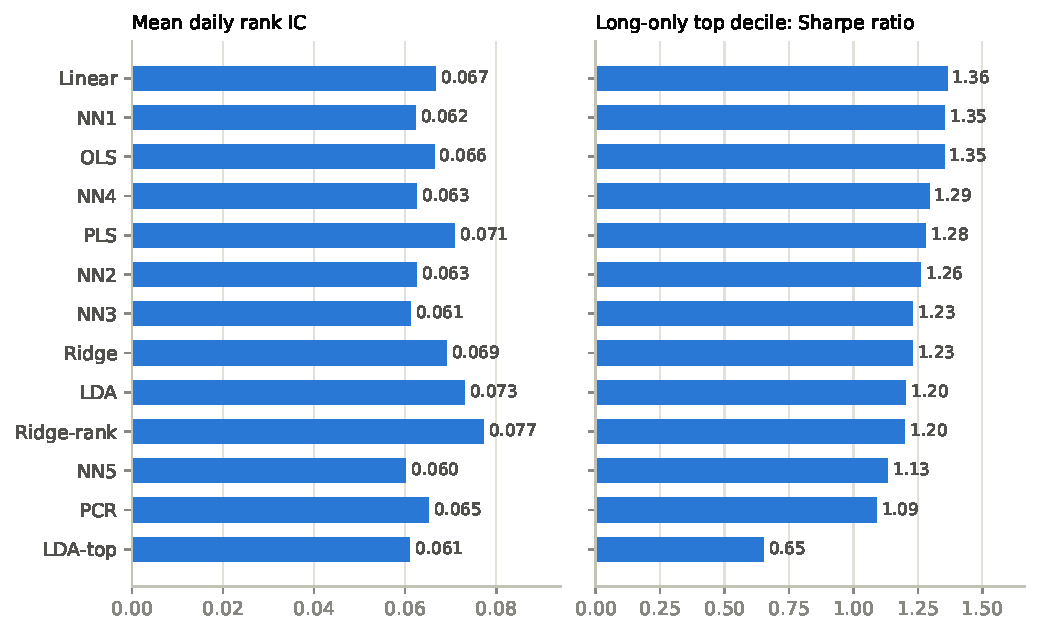
\includegraphics[width=\linewidth]{figures/fig_ic_vs_sharpe.pdf}\\[2pt]
\footnotesize (a) Rank IC and long-only Sharpe ratio; orange models are trained end to end.
\end{minipage}\hfill
\begin{minipage}[c]{0.51\linewidth}\centering
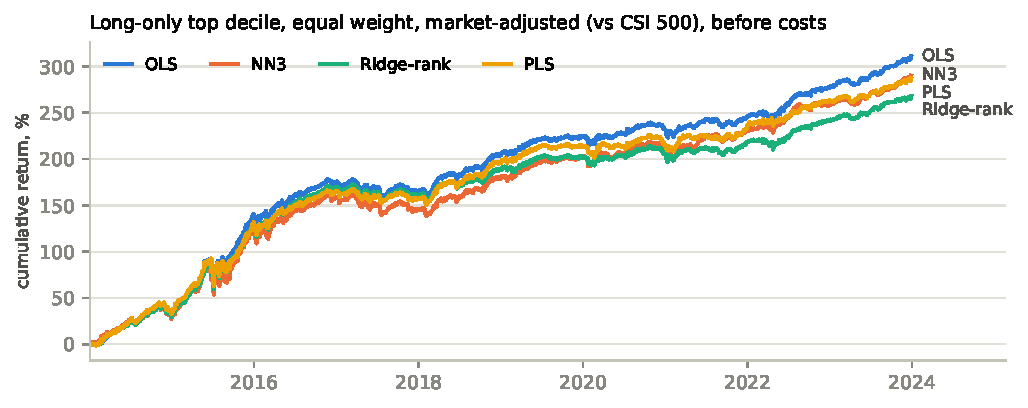
\includegraphics[width=\linewidth]{figures/fig_cumulative.pdf}\\[2pt]
\footnotesize (b) Cumulative market-adjusted return of the long-only top decile.
\end{minipage}
\caption{Statistical accuracy versus portfolio quality, 2014--2023.}\label{fig:ic}\label{fig:cum}
\end{figure}

\paragraph{Accuracy is not decision quality.} Among two-stage models, ridge on return ranks, linear SVR and LDA
have the highest rank ICs (0.077, 0.075, 0.073), yet the linear model fit by MSE has the best long-only Sharpe
ratio (1.36). E2E training makes the point directly: it lowers every model's rank IC (NN3 from 0.061 to 0.056,
ridge from 0.069 to 0.053) while raising its top-decile return (Figure~\ref{fig:ic}a).

\paragraph{End-to-end learning.} E2E raises the long-only return of NN3 by 2.5 points a year ($t=1.69$,
one-sided $p=0.05$, two-sided $p=0.09$) and of ridge by 4.1 points ($t=2.17$), adds little to the linear model
(+0.7) and lowers the GMM experts ($-2.1$). Once trained for the decision, the network no longer trails the
linear model (NN3 Sharpe ratio from 1.23 to 1.35), but the gains are far smaller than the paper's. The warm start
is not doing the work: on the first eight windows NN3 trained from scratch reaches a Sharpe ratio of 1.79,
against 1.84 when warm-started and 1.67 for the two-stage model.

\paragraph{Decision-aware PCA.} Twenty principal components are a poor basis for a linear model (Sharpe ratio
1.00, the lowest in its family). Letting the portfolio objective move the loadings raises its return from 21.8\%
to 30.4\% a year (Sharpe ratio 1.36, $t=4.96$), level with the full 251-feature model. The two decision-aware
PCA20-Linear comparisons are the only ones in Table~\ref{tab:e2e} that survive a Holm adjustment for the nine
tests. We did not run E2E with the PCA loadings fixed for this model, so the gain combines E2E training of the
head with the moving loadings. For NN3 the effect is small (+1.4 points, $t=1.03$), and a stronger pull toward
PCA ($\mu=1$) helps less than $\mu=0.1$.

\paragraph{Other reductions and mixtures.} For NN3 the choice of reduction matters little (Sharpe ratio 1.24 with
PCA, 1.19 with LDA, 1.01 with PLS), and none beats the full feature set. The persistence-aware basis cuts daily
turnover from about 30\% to 3\% but loses most of the signal (IC 0.021). The GMM mixture of experts (Sharpe ratio
1.27) is matched by hard size terciles (1.36): its gain comes from separating large and small firms, which a size
split already does.

\paragraph{Transaction costs.} At 20 bps, NN3 trained with costs earns 24.7\% a year net of costs (Sharpe ratio
1.07) with 7\% daily turnover. The MSE top decile earns 15.2\% with 28\% turnover ($t=7.27$ for the difference),
the cost-aware optimizer fed MSE forecasts (MSE-Opt) 22.1\% ($t=2.09$), and MSE-Opt with its cost penalty tuned on
validation 23.2\% ($t=1.23$). Much of E2E's lead over the paper's MSE-Opt benchmark thus reflects the benchmark's
mis-scaled forecasts (Table~\ref{tab:audit}).

\paragraph{Mean--SD utility.} With $\eta=1$ and a 10\% cap, the mean--SD E2E network earns 30.0\% a year at 22.1\%
volatility (Sharpe ratio 1.36), against 29.5\% and 23.0\% (1.28) when the same problem is solved with the MSE
forecasts; the difference is not significant ($t=0.30$).

\paragraph{Size and tradability.} Without the bottom 30\% by market capitalization the linear model earns 22.8\%
(Sharpe ratio 1.03; the paper: 28.0\%, 1.44). Without our tradability rules the same models earned over 50\% a
year. The average stock beat the mid-cap CSI 500 by 2.4\% a year, so part of every return is a size effect.

\section{Conclusion}
On free China A-share data with explicit tradability rules, training for the decision instead of for accuracy
improves long-only portfolios, but by less than Wang et al.\ report, and mainly for models that are weak under
MSE. The clearest gain comes from decision-aware PCA, which turns the weakest linear model into one of the best.
With costs, E2E training sharply cuts turnover, but a properly tuned two-stage benchmark closes most of the gap,
so claims of dominance should be tested against such benchmarks. This round covers one cost level (20 bps) and
one risk aversion ($\eta=1$); the full grids, the PPP benchmark and the persistence-aware basis under costs are
implemented and left for the next round. Code: see the accompanying repository.

\begin{multicols}{2}
\begin{thebibliography}{9}\scriptsize\setlength{\itemsep}{0pt}\setlength{\parskip}{0pt}
\bibitem{wang} Wang, Y., Gao, H., Harvey, C.\,R., Liu, Y., Tao, X. (2026). Machine learning meets Markowitz. Working paper, SSRN 5947774.
\bibitem{gkx} Gu, S., Kelly, B., Xiu, D. (2020). Empirical asset pricing via machine learning. \emph{Review of Financial Studies} 33(5), 2223--2273.
\bibitem{amos} Amos, B., Kolter, J.\,Z. (2017). OptNet: differentiable optimization as a layer in neural networks. \emph{ICML}.
\bibitem{dejong} de Jong, S. (1993). SIMPLS: an alternative approach to partial least squares regression. \emph{Chemometrics and Intelligent Laboratory Systems} 18, 251--263.
\bibitem{lwz} Leippold, M., Wang, Q., Zhou, W. (2022). Machine learning in the Chinese stock market. \emph{Journal of Financial Economics} 145(2), 64--82.
\bibitem{lsy} Liu, J., Stambaugh, R.\,F., Yuan, Y. (2019). Size and value in China. \emph{Journal of Financial Economics} 134(1), 48--69.
\bibitem{hlz} Harvey, C.\,R., Liu, Y., Zhu, H. (2016). \ldots and the cross-section of expected returns. \emph{Review of Financial Studies} 29(1), 5--68.
\end{thebibliography}
\end{multicols}
\end{document}
